\chapter{Psalm 22}

\begin{figure}
  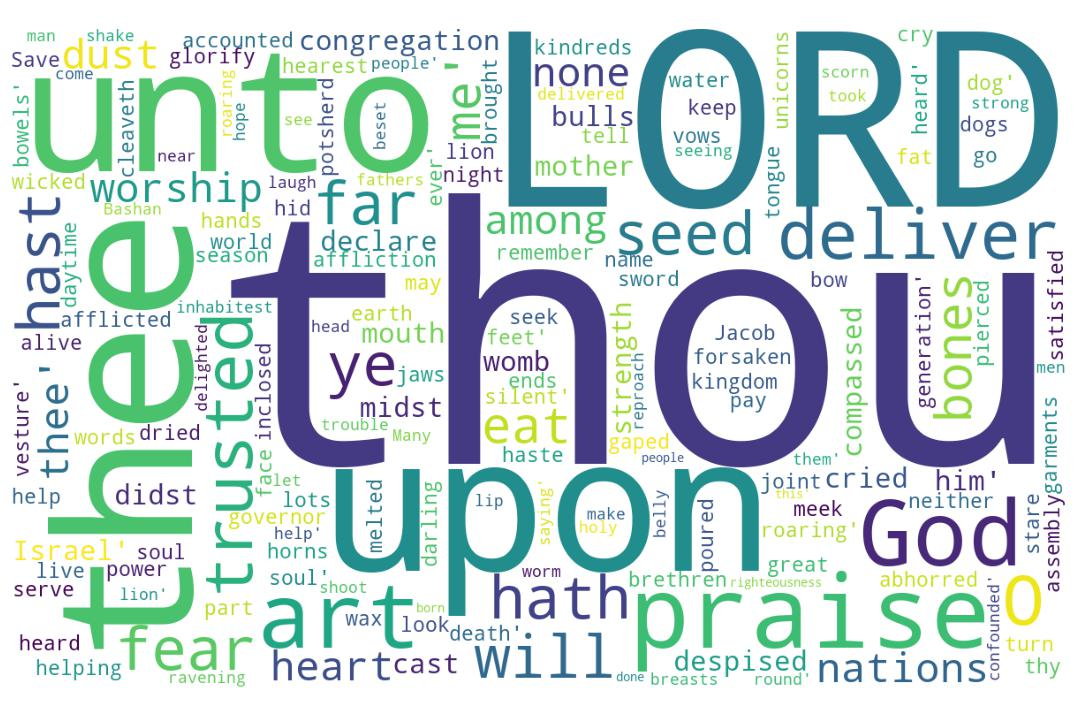
\includegraphics[width=\linewidth]{19OT-Psalms/Psalm22-WordCloud.jpg}
  \caption{Psalm 22 Word Cloud}
  \label{fig:Psalm 22 word Cloud}
\end{figure}

\marginpar{\scriptsize \centering \fcolorbox{bone}{lime}{\textbf{NOW COMES JESUS}}\\ (Psalm 22:1--31) \begin{compactenum}[I.][8]
    \item \textbf{Words of God's Roaring} \index[scripture]{Psalms!Psa 022:01} (Psa 22:1)
    \item The \textbf{Wounds of Suffering} 
    \item The \textbf{Worm of Sin} \index[scripture]{Psalms!Psa 022:06} (Psa  22:6)
    \item The \textbf{Womb of a Servant} \index[scripture]{Psalms!Psa 022:09--10} (Psal 22:9--10)
    \item The \textbf{Wicked that Encompassed him} \index[scripture]{Psalms!Psa 022:12}\index[scripture]{Psalms!Psa 022:16} (Psa 22:12, 16)
    \item The \textbf{World that will Remember} \index[scripture]{Psalms!Psa 022:27} (Psa 22:27)
    \item The \textbf{Ones who will Come} \index[scripture]{Psalms!Psa 022:30}\index[scripture]{Psalms!Psa 022:31} (Psa 22:30, 31)
\end{compactenum}}

\marginpar{\scriptsize \centering \fcolorbox{bone}{yellow}{\textbf{SEVEN LOOKS}}\\ (Psalm 22:1--31) \begin{compactenum}[I.][8]
    \item The \textbf{Upward Look} \index[scripture]{Psalms!Psa 022:01-03} (Psa 22:1--3) 
    \item The \textbf{Backward Look} \index[scripture]{Psalms!Psa 022:04-06} (Psa 22:4--6) 
    \item The \textbf{Outward Look} \index[scripture]{Psalms!Psa 022:07-08} (Psa 22:7--8) 
    \item The \textbf{Inward Look} \index[scripture]{Psalms!Psa 022:14-17} (Psa 22:14--17) 
    \item The \textbf{Downward Look} \index[scripture]{Psalms!Psa 022:18} (Psa 22:18) 
    \item The \textbf{Onward Look} \index[scripture]{Psalms!Psa 022:22} (Psa 22:22) 
    \item The \textbf{Millennial Look} %(Psalm) 
\end{compactenum}}

\marginpar{\scriptsize \centering \fcolorbox{bone}{black}{\textbf{\textcolor[cmyk]{0,0,0,0}{THE WORK ON THE CROSS}}}\\ (Psalm 22:1--31) 
\begin{compactenum}[I.][8]
    \item The \textbf{Separation}  \index[scripture]{Psalms!Psa 022:01}(Psa 22:1) 
    \item The \textbf{Sin} \index[scripture]{Psalms!Psa 022:06}(Psa 22:6)
    \item The \textbf{Scorn} \index[scripture]{Psalms!Psa 022:07}(Psa 22:7)
    \item The \textbf{Strength} \index[scripture]{Psalms!Psa 022:15}(Psa 22:15) 
    \item The \textbf{Season} 
    \item The \textbf{Speech} \index[scripture]{Psalms!Psa 022:22}(Psa 22:22) 
    \item The \textbf{Satisfaction} \index[scripture]{Psalms!Psa 022:26}(Psa 22:26) 
    \item The \textbf{Seed} \index[scripture]{Psalms!Psa 022:30}\index[scripture]{Psalms!Psa 022:31}(Psa 22:30, 31) 
\end{compactenum}}

\marginpar{\scriptsize \centering \fcolorbox{bone}{blue}{\textbf{\textcolor[cmyk]{0,0,0,0}{THE SALVATION NARRATIVE}}}\\ (Psalm 22:1--31) 
\begin{compactenum}[I.][8]
    \item \textbf{Cry of Separation} - (Psa 22:1-5)
    \item \textbf{Cost of Sin} - (Psa 22: 6)  
    \item \textbf{Compassion Seen} - (Psa 22:12, 16)
    \item \textbf{Congregation of the Saints} - (Psa 22: 22, 25)
    \item \textbf{Call of the Saved} - (Psa 22: 23)
    \item \textbf{Concern of the Sovereign} \index[scripture]{Psalms!Psa 022:24} (Psa 22:24)
    \item \textbf{Conclusion of the Story}  - (Psa 22:27-31)
\end{compactenum}}

\marginpar{\scriptsize \centering \fcolorbox{bone}{orange}{\textbf{\textcolor[cmyk]{0,0,0,0}{THE PERSON OF CHRIST}}}\\ (Psalm 22:1--31) \begin{compactenum}[I.][8]
    \item was \textbf{Devoid of God's help} - - completely abandoned by God as he became sin
    \item was on \textbf{Display to the mockers} 
    \item was \textbf{Despised by the people} -- as a fool
    \item was \textbf{Disrobed and naked}  (completed dishonored)
    \item was \textbf{Depleted of energy, emotions, and dignity} 
    \item was \textbf{Distressed and pierced} (Verse 11)
    \item was \textbf{Dying for all sin, past and future} 
\end{compactenum}}

\footnote{\textcolor[cmyk]{0.99998,1,0,0}{\hyperlink{TOC}{Return to end of Table of Contents.}}}\footnote{\href{https://www.audioverse.org/english/audiobibles/books/ENGKJV/O/Ps/1}{\textcolor[cmyk]{0.99998,1,0,0}{Psalms Audio}}}\textcolor[cmyk]{0.99998,1,0,0}{To the chief Musician upon Aijeleth Shahar, A Psalm of David.}\\
\\
\textcolor[cmyk]{0.99998,1,0,0}{My God, my God, why hast thou forsaken me? \emph{why} \emph{art} \emph{thou} \emph{so} far from helping me, \emph{and} \emph{from} the \fcolorbox{bone}{lime}{words of my roaring}?}\footnote{\textbf{Matthew 27:46} - And about the ninth hour Jesus cried with a loud voice, saying, Eli, Eli, lama sabachthani? that is to say, My God, my God, why hast thou forsaken me?}\footnote{\textbf{Mark 15:34} - And at the ninth hour Jesus cried with a loud voice, saying, Eloi, Eloi, lama sabachthani? which is, being interpreted, My God, my God, why hast thou forsaken me?}
[2] \textcolor[cmyk]{0.99998,1,0,0}{O my God, I cry in the daytime, but thou hearest not; and in the night season, and am not silent.}\footnote{\textbf{Psalm 42:3} - My tears have been my meat day and night, while they continually say unto me, Where is thy God?}\footnote{\textbf{Psalm 55:16-17} - As for me, I will call upon God; and the LORD shall save me. [17] Evening, and morning, and at noon, will I pray, and cry aloud: and he shall hear my voice.}\footnote{\textbf{Psalm 88:1} - O LORD God of my salvation, I have cried day and night before thee:}\footnote{\textbf{Luke 18:7} -And shall not God avenge his own elect, which cry day and night unto him, though he bear long with them?}\footnote{\textbf{1 Thessalonians 3:10} - Night and day praying exceedingly that we might see your face, and might perfect that which is lacking in your faith?}\footnote{\textbf{2 Timothy 1:3} - I thank God, whom I serve from my forefathers with pure conscience, that without ceasing I have remembrance of thee in my prayers night and day;}
[3] \textcolor[cmyk]{0.99998,1,0,0}{But thou \emph{art} holy, \emph{O} \emph{thou} that inhabitest the praises of Israel.}\footnote{\textbf{Psalm 145:17} - The LORD is righteous in all his ways, and holy in all his works.}\footnote{\textbf{Isaiah 6:3} - And one cried unto another, and said, Holy, holy, holy, is the LORD of hosts: the whole earth is full of his glory.}\footnote{\textbf{Revelation 4:8} - And the four beasts had each of them six wings about him; and they were full of eyes within: and they rest not day and night, saying, Holy, holy, holy, Lord God Almighty, which was, and is, and is to come.}
[4] \textcolor[cmyk]{0.99998,1,0,0}{Our fathers trusted in thee: they trusted, and thou didst deliver them.}\footnote{\textbf{Genesis 15:6} - And he believed in the LORD; and he counted it to him for righteousness.}
[5] \textcolor[cmyk]{0.99998,1,0,0}{They cried unto thee, and were delivered: they trusted in thee, and were not confounded.}\footnote{\textbf{Psalm 25:2-3} - O my God, I trust in thee: let me not be ashamed, let not mine enemies triumph over me. [3] Yea, let none that wait on thee be ashamed: let them be ashamed which transgress without cause.}\footnote{\textbf{Isaiah 45:17} - But Israel shall be saved in the LORD with an everlasting salvation: ye shall not be ashamed nor confounded world without end.}\footnote{\textbf{1 Peter 2:6} - Wherefore also it is contained in the scripture, Behold, I lay in Sion a chief corner stone, elect, precious: and he that believeth on him shall not be confounded.}
[6] \textcolor[cmyk]{0.99998,1,0,0}{But I \emph{am} \fcolorbox{bone}{lime}{a worm}, and no man; a reproach of men, and despised of the people.}\footnote{\textbf{Job 25:6} - How much less man, that is a worm? and the son of man, which is a worm?}\footnote{\textbf{Isaiah 41:14} - Fear not, thou worm Jacob, and ye men of Israel; I will help thee, saith the LORD, and thy redeemer, the Holy One of Israel.}\footnote{\textbf{Lamentations 3:30} - He giveth his cheek to him that smiteth him: he is filled full with reproach.}
[7] \textcolor[cmyk]{0.99998,1,0,0}{All they that see me laugh me to scorn: they shoot out the lip, they shake the head, \emph{saying},}\footnote{\textbf{Job 16:10} - They have gaped upon me with their mouth; they have smitten me upon the cheek reproachfully; they have gathered themselves together against me.}\footnote{\textbf{Job 30:9-11} - And now am I their song, yea, I am their byword. [10] They abhor me, they flee far from me, and spare not to spit in my face. [11] Because he hath loosed my cord, and afflicted me, they have also let loose the bridle before me.}\footnote{\textbf{Psalm 44:14} - Thou makest us a byword among the heathen, a shaking of the head among the people.}\footnote{\textbf{Psalm 109:25} - I became also a reproach unto them: when they looked upon me they shaked their heads.}\footnote{\textbf{Isaiah 37:22-23} - This is the word which the LORD hath spoken concerning him; The virgin, the daughter of Zion, hath despised thee, and laughed thee to scorn; the daughter of Jerusalem hath shaken her head at thee. [23] Whom hast thou reproached and blasphemed? and against whom hast thou exalted thy voice, and lifted up thine eyes on high? even against the Holy One of Israel.}
[8] \textcolor[cmyk]{0.99998,1,0,0}{He trusted on the LORD \emph{that} he would deliver black{him}: let \fcolorbox{bone}{bone}{him} deliver \fcolorbox{bone}{bone}{him}, seeing he delighted in \fcolorbox{bone}{bone}{him}.}\footnote{\textbf{Psalm 42:10} - As with a sword in my bones, mine enemies reproach me; while they say daily unto me, Where is thy God?}\footnote{\textbf{Isaiah 42:1} - Behold my servant, whom I uphold; mine elect, in whom my soul delighteth; I have put my spirit upon him: he shall bring forth judgment to the Gentiles.}\footnote{\textbf{Matthew 27:42-43} - He saved others; himself he cannot save. If he be the King of Israel, let him now come down from the cross, and we will believe him. [43] He trusted in God; let him deliver him now, if he will have him: for he said, I am the Son of God.}
[9] \textcolor[cmyk]{0.99998,1,0,0}{But thou \emph{art} he that took me out of the \fcolorbox{bone}{lime}{womb}: thou didst make me hope \emph{when} \emph{I} \emph{was} upon my mother's breasts.}\footnote{\textbf{Psalm 7:16} - By thee have I been holden up from the womb: thou art he that took me out of my mother's bowels: my praise shall be continually of thee.}
[10] \textcolor[cmyk]{0.99998,1,0,0}{I was cast upon thee from the womb: thou \emph{art} my God from my mother's belly.}\footnote{\textbf{Isaiah 46:3-4} - Hearken unto me, O house of Jacob, and all the remnant of the house of Israel, which are borne by me from the belly, which are carried from the womb: [4] And even to your old age I am he; and even to hoar hairs will I carry you: I have made, and I will bear; even I will carry, and will deliver you.}
[11] \textcolor[cmyk]{0.99998,1,0,0}{Be not far from me; for trouble \emph{is} near; for \emph{there} \emph{is} none to help.}\footnote{\textbf{Psalm 10:1} - Why standest thou afar off, O LORD? why hidest thou thyself in times of trouble?}\footnote{\textbf{Psalm 13:1-3} - How long wilt thou forget me, O LORD? for ever? how long wilt thou hide thy face from me? [2] How long shall I take counsel in my soul, having sorrow in my heart daily? how long shall mine enemy be exalted over me? [3] Consider and hear me, O LORD my God: lighten mine eyes, lest I sleep the sleep of death;}
[12] \textcolor[cmyk]{0.99998,1,0,0}{Many \fcolorbox{bone}{lime}{bulls} have compassed me: strong \emph{bulls} of Bashan have beset me round.}\footnote{\textbf{Deuteronomy 32:1-15} - Butter of kine, and milk of sheep, with fat of lambs, and rams of the breed of Bashan, and goats, with the fat of kidneys of wheat; and thou didst drink the pure blood of the grape. [15] But Jeshurun waxed fat, and kicked: thou art waxen fat, thou art grown thick, thou art covered with fatness; then he forsook God which made him, and lightly esteemed the Rock of his salvation.}\footnote{\textbf{Ezekiel 39:18} - Ye shall eat the flesh of the mighty, and drink the blood of the princes of the earth, of rams, of lambs, and of goats, of bullocks, all of them fatlings of Bashan.}\footnote{\textbf{Amos 4:1-3} - Hear this word, ye kine of Bashan, that are in the mountain of Samaria, which oppress the poor, which crush the needy, which say to their masters, Bring, and let us drink. [2] The Lord GOD hath sworn by his holiness, that, lo, the days shall come upon you, that he will take you away with hooks, and your posterity with fishhooks. [3] And ye shall go out at the breaches, every cow at that which is before her; and ye shall cast them into the palace, saith the LORD.}
[13] \textcolor[cmyk]{0.99998,1,0,0}{They gaped upon me \emph{with} their mouths, \emph{as} a ravening and a roaring lion.}\footnote{\textbf{Psalm 35:21} - Yea, they opened their mouth wide against me, and said, Aha, aha, our eye hath seen it.}\footnote{\textbf{Job 16:10} - They have gaped upon me with their mouth; they have smitten me upon the cheek reproachfully; they have gathered themselves together against me.}\footnote{\textbf{Lamentations 2:16} - All thine enemies have opened their mouth against thee: they hiss and gnash the teeth: they say, We have swallowed her up: certainly this is the day that we looked for; we have found, we have seen it.}\footnote{\textbf{Lamentations 3:46} - All our enemies have opened their mouths against us.}\footnote{\textbf{1 Peter 5:8} - Be sober, be vigilant; because your adversary the devil, as a roaring lion, walketh about, seeking whom he may devour:}
[14] \textcolor[cmyk]{0.99998,1,0,0}{I am poured out like water, and all my bones are out of joint: my heart is like wax; it is melted in the midst of my bowels.}
[15] \textcolor[cmyk]{0.99998,1,0,0}{My strength is dried up like a potsherd; and my tongue cleaveth to my jaws; and thou hast brought me into the dust of death.}\footnote{\textbf{Psalm 69:3, 21} - I am weary of my crying: my throat is dried: mine eyes fail while I wait for my God. [21] They gave me also gall for my meat; and in my thirst they gave me vinegar to drink.}\footnote{\textbf{Job 29:10} - The nobles held their peace, and their tongue cleaved to the roof of their mouth.}\footnote{\textbf{Lamentations 4:4} - The tongue of the sucking child cleaveth to the roof of his mouth for thirst: the young children ask bread, and no man breaketh it unto them.}\footnote{\textbf{Job 7:21} - And why dost thou not pardon my transgression, and take away mine iniquity? for now shall I sleep in the dust; and thou shalt seek me in the morning, but I shall not be.}\footnote{\textbf{Job 10:9} -  Remember, I beseech thee, that thou hast made me as the clay; and wilt thou bring me into dust again?}\footnote{\textbf{Job 34:15} - All flesh shall perish together, and man shall turn again unto dust.}
[16] \textcolor[cmyk]{0.99998,1,0,0}{For dogs have compassed me: the assembly of the wicked have inclosed me: they pierced my hands and my feet.}\footnote{\textbf{Zechariah 12:10} - And I will pour upon the house of David, and upon the inhabitants of Jerusalem, the spirit of grace and of supplications: and they shall look upon me whom they have pierced, and they shall mourn for him, as one mourneth for his only son, and shall be in bitterness for him, as one that is in bitterness for his firstborn.}\footnote{\textbf{Matthew 27:35} - And they crucified him, and parted his garments, casting lots: that it might be fulfilled which was spoken by the prophet, They parted my garments among them, and upon my vesture did they cast lots.}
[17] \textcolor[cmyk]{0.99998,1,0,0}{I may tell all my bones: they look \emph{and} stare upon me.}\footnote{\textbf{Psalm 102:3-5} - For my days are consumed like smoke, and my bones are burned as an hearth. [4] My heart is smitten, and withered like grass; so that I forget to eat my bread. [5] By reason of the voice of my groaning my bones cleave to my skin.}\footnote{\textbf{Job 33:21} - His flesh is consumed away, that it cannot be seen; and his bones that were not seen stick out.}\footnote{\textbf{Isaiah 52:14} - As many were astonied at thee; his visage was so marred more than any man, and his form more than the sons of men:}
[18] \textcolor[cmyk]{0.99998,1,0,0}{They part my garments among them, and cast lots upon my vesture.}\footnote{\textbf{Matthew 27:35} - And they crucified him, and parted his garments, casting lots: that it might be fulfilled which was spoken by the prophet, They parted my garments among them, and upon my vesture did they cast lots.}\footnote{\textbf{Mark 15:24} - And when they had crucified him, they parted his garments, casting lots upon them, what every man should take.}\footnote{\textbf{Luke 23:34} - Then said Jesus, Father, forgive them; for they know not what they do. And they parted his raiment, and cast lots.}\footnote{\textbf{John 19:23-24} - Then the soldiers, when they had crucified Jesus, took his garments, and made four parts, to every soldier a part; and also his coat: now the coat was without seam, woven from the top throughout. [24] They said therefore among themselves, Let us not rend it, but cast lots for it, whose it shall be: that the scripture might be fulfilled, which saith, They parted my raiment among them, and for my vesture they did cast lots. These things therefore the soldiers did.}
[19] \textcolor[cmyk]{0.99998,1,0,0}{But be not thou far from me, O LORD: O my strength, haste thee to help me.}\footnote{\textbf{Psalm 18:1} - I will love thee, O LORD, my strength.}\footnote{\textbf{Psalm 21:1} - The king shall joy in thy strength, O LORD; and in thy salvation how greatly shall he rejoice!}\footnote{\textbf{Psalm 40:17} - But I am poor and needy; yet the Lord thinketh upon me: thou art my help and my deliverer; make no tarrying, O my God.}
[20] \textcolor[cmyk]{0.99998,1,0,0}{Deliver my soul from the sword; my darling from the power of the dog.}\footnote{\textbf{Psalm 17:13} - Arise, O LORD, disappoint him, cast him down: deliver my soul from the wicked, which is thy sword:}\footnote{\textbf{Zechariah 13:7} - Awake, O sword, against my shepherd, and against the man that is my fellow, saith the LORD of hosts: smite the shepherd, and the sheep shall be scattered: and I will turn mine hand upon the little ones.}\footnote{\textbf{Psalm 35:17} - Lord, how long wilt thou look on? rescue my soul from their destructions, my darling from the lions.}
[21] \textcolor[cmyk]{0.99998,1,0,0}{Save me from the lion's mouth: for thou hast heard me from the horns of the unicorns.}\footnote{\textbf{Numbers 23:22} - God brought them out of Egypt; he hath as it were the strength of an unicorn.}\footnote{\textbf{Deuteronomy 33:17} - His glory is like the firstling of his bullock, and his horns are like the horns of unicorns: with them he shall push the people together to the ends of the earth: and they are the ten thousands of Ephraim, and they are the thousands of Manasseh.}
[22] \textcolor[cmyk]{0.99998,1,0,0}{I will declare thy name unto my brethren: in the midst of the congregation will praise thee.}\footnote{\textbf{Psalm 40:9-10} - I have preached righteousness in the great congregation: lo, I have not refrained my lips, O LORD, thou knowest. [10] I have not hid thy righteousness within my heart; I have declared thy faithfulness and thy salvation: I have not concealed thy lovingkindness and thy truth from the great congregation.}
[23] \textcolor[cmyk]{0.99998,1,0,0}{Ye that fear the LORD, praise \fcolorbox{bone}{bone}{him}; all ye the seed of Jacob, glorify \fcolorbox{bone}{bone}{him}; and fear \fcolorbox{bone}{bone}{him}, all ye the seed of Israel.}\footnote{\textbf{Psalm 115:11} - Ye that fear the LORD, trust in the LORD: he is their help and their shield.}
[24] \textcolor[cmyk]{0.99998,1,0,0}{For he hath not despised nor abhorred the affliction of the afflicted; neither hath he hid his face from \fcolorbox{bone}{bone}{him}; but when he cried unto \fcolorbox{bone}{bone}{him}, he heard.}\footnote{\textbf{Isaiah 50:6-9} - I gave my back to the smiters, and my cheeks to them that plucked off the hair: I hid not my face from shame and spitting. [7] For the Lord GOD will help me; therefore shall I not be confounded: therefore have I set my face like a flint, and I know that I shall not be ashamed. [8] He is near that justifieth me; who will contend with me? let us stand together: who is mine adversary? let him come near to me. [9] Behold, the Lord GOD will help me; who is he that shall condemn me? lo, they all shall wax old as a garment; the moth shall eat them up.}
[25] \textcolor[cmyk]{0.99998,1,0,0}{My praise \emph{shall} \emph{be} of thee in the great congregation: I will pay my vows before them that fear \fcolorbox{bone}{bone}{him}.}\footnote{\textbf{Psalm 56:12} - Thy vows are upon me, O God: I will render praises unto thee.}\footnote{\textbf{Psalm 65:1} - Praise waiteth for thee, O God, in Sion: and unto thee shall the vow be performed.}\footnote{\textbf{Psalm 66:13, 16} - I will go into thy house with burnt offerings: I will pay thee my vows, [16] Come and hear, all ye that fear God, and I will declare what he hath done for my soul.}\footnote{\textbf{Ecclesiastes 5:4-5} - When thou vowest a vow unto God, defer not to pay it; for he hath no pleasure in fools: pay that which thou hast vowed. [5] Better is it that thou shouldest not vow, than that thou shouldest vow and not pay.}\footnote{\textbf{1 Kings 8:65} - And at that time Solomon held a feast, and all Israel with him, a great congregation, from the entering in of Hamath unto the river of Egypt, before the LORD our God, seven days and seven days, even fourteen days.}\footnote{\textbf{2 Chronicles 7:8} - Also at the same time Solomon kept the feast seven days, and all Israel with him, a very great congregation, from the entering in of Hamath unto the river of Egypt.}\footnote{\textbf{2 Choronciles 30:13} - And there assembled at Jerusalem much people to keep the feast of unleavened bread in the second month, a very great congregation.}\footnote{\textbf{Ezra 10:1} - Now when Ezra had prayed, and when he had confessed, weeping and casting himself down before the house of God, there assembled unto him out of Israel a very great congregation of men and women and children: for the people wept very sore.}
[26] \textcolor[cmyk]{0.99998,1,0,0}{The meek shall eat and be satisfied: they shall praise the LORD that seek \fcolorbox{bone}{bone}{him}: your heart shall live for ever.}\footnote{\textbf{Psalm 69:32} - The humble shall see this, and be glad: and your heart shall live that seek God.}
[27] \textcolor[cmyk]{0.99998,1,0,0}{All the ends of the \fcolorbox{bone}{lime}{world} shall remember and turn unto the LORD: and all the kindreds of the nations shall worship before thee.}\footnote{\textbf{Acts 14:15} - And saying, Sirs, why do ye these things? We also are men of like passions with you, and preach unto you that ye should turn from these vanities unto the living God, which made heaven, and earth, and the sea, and all things that are therein:}\footnote{\textbf{Acts 20:21} - Testifying both to the Jews, and also to the Greeks, repentance toward God, and faith toward our Lord Jesus Christ.}\footnote{\textbf{Acts 26:18-20} - To open their eyes, and to turn them from darkness to light, and from the power of Satan unto God, that they may receive forgiveness of sins, and inheritance among them which are sanctified by faith that is in me. [19] Whereupon, O king Agrippa, I was not disobedient unto the heavenly vision: [20] But shewed first unto them of Damascus, and at Jerusalem, and throughout all the coasts of Judaea, and then to the Gentiles, that they should repent and turn to God, and do works meet for repentance.}\footnote{\textbf{1 Thessalonians 1:9} - For they themselves shew of us what manner of entering in we had unto you, and how ye turned to God from idols to serve the living and true God;}
[28] \textcolor[cmyk]{0.99998,1,0,0}{For the kingdom \emph{is} the LORD'S: and he \emph{is} the governor among the nations.}\footnote{\textbf{Psalm 47:7-8} - For God is the King of all the earth: sing ye praises with understanding. [8] God reigneth over the heathen: God sitteth upon the throne of his holiness.}\footnote{\textbf{Daniel 7:14} -And there was given him dominion, and glory, and a kingdom, that all people, nations, and languages, should serve him: his dominion is an everlasting dominion, which shall not pass away, and his kingdom that which shall not be destroyed.}\footnote{\textbf{Obadiah 1:21} - And saviours shall come up on mount Zion to judge the mount of Esau; and the kingdom shall be the LORD'S.}\footnote{\textbf{Zechariah 14:9} - And the LORD shall be king over all the earth: in that day shall there be one LORD, and his name one.}\footnote{\textbf{Matthew 6:13} - And lead us not into temptation, but deliver us from evil: For thine is the kingdom, and the power, and the glory, for ever. Amen.}\footnote{\textbf{Revelation 11:15} - And the seventh angel sounded; and there were great voices in heaven, saying, The kingdoms of this world are become the kingdoms of our Lord, and of his Christ; and he shall reign for ever and ever.}
[29] \textcolor[cmyk]{0.99998,1,0,0}{All \emph{they} \emph{that} \emph{be} fat upon earth shall eat and worship: all they that go down to the dust shall bow before \fcolorbox{bone}{bone}{him}: and none can keep alive his own soul.}
[30] \textcolor[cmyk]{0.99998,1,0,0}{A seed shall serve \fcolorbox{bone}{bone}{him}; it shall be \fcolorbox{bone}{lime}{accounted} to the Lord for a generation.}\footnote{\textbf{1 Peter 2:9} - But ye are a chosen generation, a royal priesthood, an holy nation, a peculiar people; that ye should shew forth the praises of him who hath called you out of darkness into his marvellous light:}
[31] \textcolor[cmyk]{0.99998,1,0,0}{They shall come, and shall declare his righteousness unto a people that shall be born, that he hath done \emph{this}.}

